
\begin{frame}
\frametitle{Perspectiva general}
%------------------------------
\begin{columns}

    \begin{column}{0.50\textwidth}
    \vspace{-5pt}
    \begin{block}{\textcolor{blue}{Oferta}}
        \begin{column}{0.1\textwidth}
        \vspace{-10pt} % estos espacios negativos son claves para alinear
            \tiny
            \begin{align*}
            c_{1,t}+\Phi_t \le y\\
            c_{2,t+1}\le\Phi_{t+1}^R\\
            N_{t-1}\textcolor{red}{x_t} \cdot \Phi_{t-1}^{\textbf{DLT}}=N_t(*)
            \end{align*}
        \end{column}
        \begin{column}{0.35\textwidth}  
            \begin{figure}[H]
            \begin{center}
             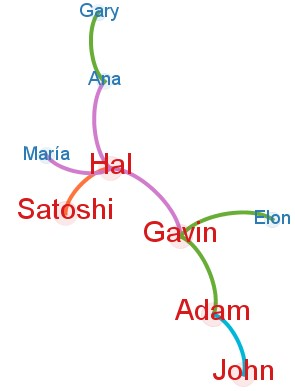
\includegraphics[width=1\textwidth]{images/C2/c2_simul_red5.jpg}
             \end{center}
            \end{figure}
            \end{column}
    \end{block}
    
    \pgfsetfillopacity{0.2}
    
    \begin{block}{Demanda}
        \vspace{-10pt}
            \tiny
              \begin{align*}
              v_{t}^{\$}{M_{t}^{\$}}&={N_{t}^{\$}\left(*\right)}+(1-\lambda_t){N_{t}^{\$}\left(*\right)}\\
              v_{t}^{\bitcoinA}{M_{t}^{\bitcoinA}}&={N_{t}^{\bitcoinA}\left(*\right)+\lambda_tN_{t}^{\$}\left(*\right)}\\
              \lambda_t&=\textcolor{blue!70}{S}(\textcolor{red}{\mu_t})
            \end{align*}
    \vspace{-20pt}
            \begin{figure}[t!]
            \begin{center}
            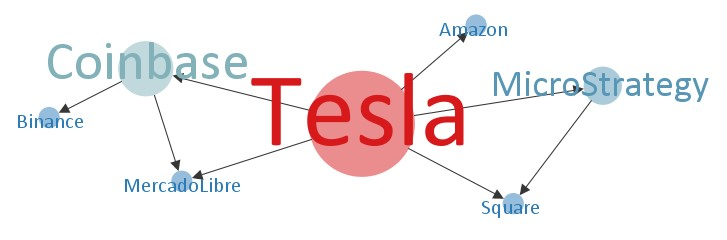
\includegraphics[width=0.6\textwidth]{images/C3/c3_simul_influ3.jpg}
             \end{center}
            \end{figure}
            
    \end{block}
    \end{column}
    
    \begin{column}{0.55\textwidth}
    
    \begin{block}{Implicancias}
    \tiny

    \begin{align*}
    v^{\$a}_1 M^{\$a}_1&=P_1^{{\$a}} + \lambda_1 (1-\alpha_1) R_1^{{\$a}} + (1-\lambda_1) \textcolor{blue!60}{\rho_1}  R_1^{{\$a}}\\
    v_1^{\$} M_1^{\$}&=(1-\lambda_1) \textcolor{green!70}{\delta_1} R_1^{\$a}\\
    v_1^{\bitcoinA} M_1^{\bitcoinA}&=\textcolor{orange}{\lambda_1}  \alpha_1 R_1^{\$a} + (1-\lambda_1) \textcolor{red}{\beta_1} R_1^{\$a}\\
    e_t^{{\$a};{\$}}&=\frac{v_1^{\$a}}{v_1^{\$}}
    \end{align*}
    
    \vspace{-5pt}
    
    \begin{figure}[H]
    \begin{center}
     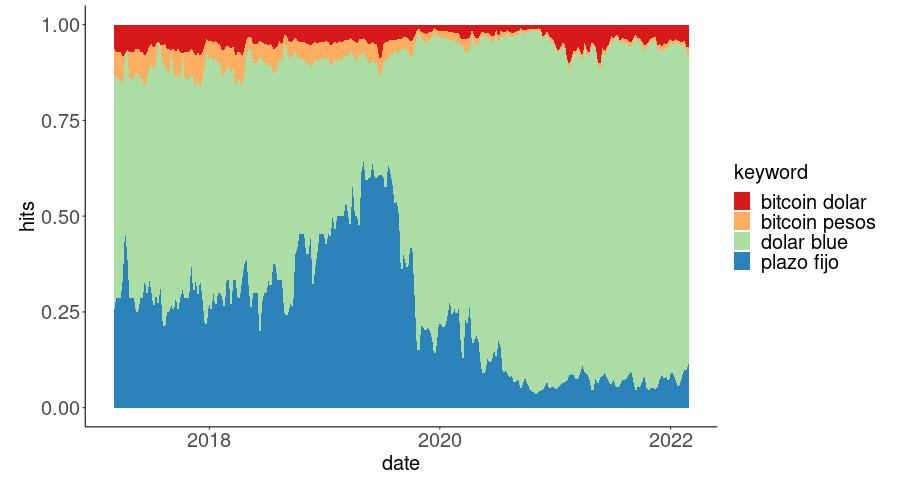
\includegraphics[width=1\textwidth]{images/C4/Rplot001.png}
     \end{center}
    \end{figure}
    
    \pgfsetfillopacity{1}
    
    \end{block}

    \end{column}
\end{columns}

\note{
\begin{itemize}
    \item Entonces, a partir de este panorama general de las diferentes partes y métodos de evaluación de la investigación, 
    \item Se comienza el análisis de la primera parte, 
    \item la cual se encuentra asociada a las características de oferta de bitcoin. 
\end{itemize}
}

\end{frame}
%----------

\subsection{Objetivos}
\begin{frame}{}

    \textcolor{blue}{\textbf{Objetivo}}.\\
    \vspace{5mm}
    \begin{itemize}
        \setlength\itemsep{1em}
        
        \item[] Describir las \textcolor{blue}{características de oferta} del sistema bitcoin.\\ 
        
        \item[] Analizar a partir de un \textcolor{blue}{modelo} si la tecnología de red distribuida puede funcionar como una tecnología equivalente al dinero.\\
        \item[] Evaluar empíricamente el modelo a partir de los \textcolor{blue}{datos de la cadena de bloques} de bitcoin.
    \end{itemize}
 
    \vspace{5mm}
    \textcolor{dgreen}{\textbf{Conjetura}}. 
    \vspace{5mm}
    \begin{itemize}
    \item[] La tecnología de red distribuida DLT que subyace al sistema bitcoin puede funcionar como una \textcolor{dgreen}{tecnología funcionalmente equivalente al dinero}.
    \end{itemize}


\note{
\begin{itemize}
    \item Para esta primera parte de la investigación, se plantean tres objetivos específicos
    \item (Leer cada objetivo)
    \item A su vez, se plantea la siguiente conjetura:
    \item (Leer la conjetura)
\end{itemize}
}
    
\end{frame}
%----------

\subsection{Definiciones}
%------------------------
\begin{frame}

\vspace{5mm}
\begin{displayquote}
El \textcolor{blue}{dinero} es equivalente a una forma primitiva de \textcolor{dgreen}{memoria}. 
\end{displayquote}
\raggedleft \cite{Kocherlakota1998} \\ \citetitle{Kocherlakota1998}

\vspace{5mm}
\begin{block}<2>{DLT como memoria}
La \textcolor{red}{DLT} es un registro público equivalente a un proceso de \textcolor{dgreen}{memoria} social. El dinero es equivalente a una forma primitiva de memoria social. Por lo tanto, una DLT sería un proceso tecnológico equivalente al \textcolor{blue}{dinero}.
\end{block}

\note{
\begin{itemize}
    \item Para esta primera parte de la investigación se propone retomar algunas \textbf{definiciones clásicas de dinero} como, por ejemplo, la idea de dinero como proceso de memoria social (a diferencia de la definición funcional clásica de dinero como medio de pago, reserva de valor o unidad de cuenta).
    \item En este sentido, \textbf{Kocherlakota} indica en "Money is Memory" que (leer cita)
    \item A partir de esa definición, se propone el siguiente concepto asociado a la DLT: (leer el recurado sobre DLT)
    \item En este marco, Shin (jefe de investigaciones en el BIS) indica que "la idea de dinero como tecnología de memoria aplicada en un registro universal era una propuesta teórica no observable". Pero que "los avances asociados a las DLT han hecho posible la existencia concreta de tal registro". Por lo tanto: "los activos digitales pueden ser considerados una tecnología equivalente al dinero"
    \href{http://www.overleaf.com}{Distributed ledgers and  the governance of money}
\end{itemize}
}
    
\end{frame}
%----------

\begin{frame}

\vspace{5mm}
\begin{displayquote}
El \textcolor{blue}{dinero} en la economía moderna es una forma especial de pagaré o, en términos económicos, un activo financiero. El dinero es un tipo especial de pagaré en el que todos tienen \textcolor{dgreen}{confianza}. 
\end{displayquote}
\raggedleft \cite{Mcleay2014c} \\ \citetitle{Mcleay2014c}

\vspace{5mm}
\begin{block}<2>{POW-confianza}
La DLT de bitcoin basa la \textcolor{dgreen}{confianza} en su sistema de registro en un mecanismo de consenso específico denominado \textcolor{red}{POW}.  \parencite{Ali2014}.
\end{block}

\note{
\begin{itemize}
    \item Una segunda definición de dinero relevante para esta primera parte de la investigación es la que asocia dinero a un proceso de confianza. 
    \item En este sentido, el Banco de Inglaterra, en una publicación muy influyente sobre la naturaleza del dinero de 2014 indica que (leer cita).
    \item A partir de este concepto, se propone un segundo concepto asociad a la DLT: (leer recuadro)
\end{itemize}
}
    
\end{frame}
%----------



\subsection{Evaluación conceptual y empírica}
%--------------------------------------------

% overview
\begin{frame}{Evaluación conceptual y empírica}
    
    \begin{block}{Modelo}
    \begin{minipage}[t][.20\textheight][t]{\textwidth}
        \begin{column}{0.30\textwidth}
        \vspace{-10pt} % estos espacios negativos son claves para alinear
            \tiny
            \begin{align*}
            {c_{1,t}+\Phi_t \le y}\\
            c_{2,t+1}\le \Phi_{t+1}^R\\
            {N_{t-1}\textcolor{red}{x_t} \cdot \Phi_{t-1}^{\textbf{DLT}}=N_t(y-c_{1,t})}
            \end{align*}
        \end{column}
        \begin{column}{0.45\textwidth}
        \end{column}
    \end{minipage}
    \end{block}

    \begin{block}{Evaluación empírica}
    
    \begin{minipage}[t][.40\textheight][t]{\textwidth}

    \begin{columns}
    \begin{column}{0.3\textwidth}
    \tiny
    \begin{figure}[H]
        \begin{center}
             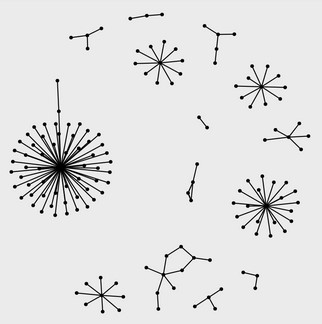
\includegraphics[width=0.8\textwidth]{images/C2/2009/sinfiltro.jpg}
         \end{center}
    \end{figure}
    \end{column}
    \begin{column}{0.3\textwidth}  
    \tiny
    \begin{figure}[H]
        \begin{center}
         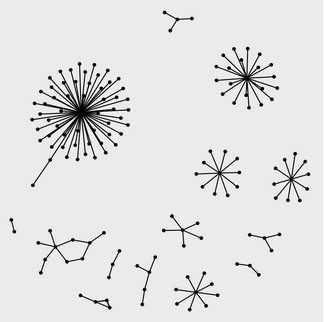
\includegraphics[width=0.75\textwidth]{images/C2/2009/filtradaa.jpg}
         \end{center}
    \end{figure}
    \end{column}
    \begin{column}{0.3\textwidth}  
    \tiny
    \begin{figure}[H]
        \begin{center}
         
\includegraphics[width=0.8\textwidth]{images/C2/2009/filtrada.jpg}
         \end{center}
    \end{figure}
    \end{column}
    \end{columns}
    \end{minipage}

    \end{block}

\note{
\begin{itemize}
    \item Evaluación conceptual: modelo OLG con registros
    \item Evaluación empírica: análisis con técnicas de red
    \end{itemize}
}

\end{frame}
%----------

% evaluación conceptual
\begin{frame}{Evaluación conceptual y empírica}
    
    \begin{block}{Modelo}
    
    \begin{minipage}[t][.20\textheight][t]{\textwidth}

        \begin{column}{0.30\textwidth}
        \vspace{-10pt} % estos espacios negativos son claves para alinear
            \tiny
            \begin{align*}
            \onslide<1,2>{c_{1,t}+\Phi_t \le y}\\
            \onslide<1,3,4>{c_{2,t+1}\le 
                \only<1,3>{\Phi_{t+1}^R}
                \only<4|handout:0>{\Phi_t \cdot x_{t+1}}}\\
            \onslide<1,5,6>{N_{t-1}\textcolor{red}{x_t} \cdot \Phi_{t-1}^{\textbf{DLT}}=N_t(y-c_{1,t})}
            \end{align*}
        \end{column}
        \begin{column}{0.45\textwidth}
            \tiny
            \only<2|handout:0>{RP1
            \begin{itemize}
                \item[] $y$: asignación de joven
                \item[] $c_{1,t}$: consumo de joven
                \item[] $\Phi_t$: regalo (DLT)
            \end{itemize}
            }
            \only<3|handout:0>{RP2
            \begin{itemize}
                \item[] $c_{2,t}$: consumo
                \item[] $\Phi_{t+1}$ regalo recibido de viejo
            \end{itemize}
            }
            \only<4>{RP2'
            \begin{itemize}
                \item[] $\Phi_{t+1} = \Phi_t \cdot x_{t+1}$
                \item[] $x_{t+1}:$ tasa de conversión
            \end{itemize}
            }
            \only<6|handout:0>{Valor de $x_t$:
            \begin{itemize}
                \item[] Con crecimiento, $x_t=\textcolor{red}{n}$
            \end{itemize}
            }
            \only<5|handout:0>{Mercado de registros (regalos)
            \begin{itemize}
                \item[] $N_t(y-c_{b,t})$: oferta de registros (regalos)
                \item[] $N_{t-1} x_t {\Phi_{t-1}}$: demanda de registros
            \end{itemize}
            }
        \end{column}
        
    \end{minipage}
    \end{block}
    
    \begin{block}{Evaluación empírica}
    
    \begin{minipage}[t][.40\textheight][t]{\textwidth}
    \end{minipage}

    \end{block}

\note{
\tiny
\begin{itemize}
    \item Para la evaluación conceptual de esta primera parte, se propone un OLG donde, en lugar de incluir un activo monetario, se incluya la DLT como sistema de registros. 
    \item RP1. $\Phi_t$: jóvenes entregan bienes a viejos (reciben a cambio un registro de esa transferencia en la DLT).
    \item RP2. Cuando se es viejo solo se puede consumir si se reciben regalos de los jóvenes. $\Phi_{t+1}$ denota los regalos recibidos cuando se es viejo. 
    \item $\Phi_t^R$ es una variable de elección; $\Phi_{t+1}^R$ es una variable dada.
    \item Se supone que un joven está dispuesto a regalar $\Phi_t$ bienes cuando es joven para obtener $\Phi_{t+1}^R$ bienes cuando es viejo.
    \item Se puede considerar que existe una tasa de conversión. Se va a indicar como $x_{t+1}$ la tasa a la cual una persona puede intercambiar unidades del bien de consumo en el período $t$ por unidades de consumo en el período $t+1$, es decir, $\Phi_t \cdot x_{t+1}=\Phi_{t+1}^R$.
    \item Si la población aumenta a una tasa constante $n$, se tiene que $x_{t+1}=n$
     
    \end{itemize}
}

\end{frame}
%----------

% evaluación empírica
\begin{frame}{Evaluación conceptual y empírica}
    
     \begin{block}{Modelo}
    \begin{minipage}[t][.20\textheight][t]{\textwidth}
        \begin{column}{0.30\textwidth}
        \vspace{-10pt} % estos espacios negativos son claves para alinear
            \tiny
            \begin{align*}
            {c_{1,t}+\Phi_t \le y}\\
            c_{2,t+1}\le \Phi_{t+1}^R\\
            {N_{t-1}\textcolor{red}{x_t} \cdot \Phi_{t-1}^{\textbf{DLT}}=N_t(y-c_{1,t})}
            \end{align*}
        \end{column}
        \begin{column}{0.45\textwidth}
        \end{column}
    \end{minipage}
    \end{block}
    
\begin{block}{Evaluación empírica}
    
    \begin{minipage}[t][.40\textheight][t]{\textwidth}

\begin{columns}
\begin{column}{0.3\textwidth}
    \tiny
    \begin{figure}[H]
        \begin{center}
             \includegraphics<1->[width=0.8\textwidth]{images/C2/2009/sinfiltro.jpg}
         \end{center}
    \end{figure}

\end{column}
\begin{column}{0.3\textwidth}  

    \tiny
    \begin{figure}[H]
        \begin{center}
         \includegraphics<2->[width=0.75\textwidth]{images/C2/2009/filtradaa.jpg}
         \end{center}
    \end{figure}

\end{column}
\begin{column}{0.3\textwidth}  

        \tiny
    \begin{figure}[H]
        \begin{center}
         \includegraphics<3>[width=0.8\textwidth]{images/C2/2009/filtrada.jpg}
         \end{center}
    \end{figure}

\end{column}
\end{columns}

    \end{minipage}

\end{block}

\note{
\tiny
\begin{itemize}
    \item Para la evaluación empírica, se busca imponen las condiciones del modelo a los datos originales de la cadena de bloques de bitcoin. 
    \item 1°se filtran las direcciones de envío (viejos) y recepción (jóvenes) que aparecen por primera vez. De esta manera se busca eliminar la posibilidad que las personas "resuciten" en períodos posteriores.
    \item 2° Solo contabiliza a los jóvenes que luego aparecen como viejos. Es decir, se impone que se cumpla la condición de efectuar regalos (nadie muere con bitcoins).
    \item Se construye una serie de tiempo con la cantidad de jóvenes de la cadena filtrada por período t
        \end{itemize}
}

\end{frame}
%----------


\subsection{Resultados}
%----------------------
% slide 1 de 3
\begin{frame}
\frametitle{Se compara el \textcolor{cyan}{valor de la red} según el modelo...}

\begin{figure}[H]
    \begin{center}
        \includegraphics<1|handout:0>[width=1\textwidth]{images/C2/c2_var_men_timesseries_presentacion_ejes.pdf}
        
        \includegraphics<2>[width=1\textwidth]{images/C2/c2_var_men_timesseries_presentacion_ejes_n.pdf}
     \end{center}
\end{figure}

\note{
\begin{itemize}
    \item Luego de generar una nueva base de datos de operaciones que cumpla con las condiciones del modelo, se construye una serie de tiempo donde se indique la cantidad de personas de cada generación. 
    \item Es decir, se está construyendo una serie que de cuenta del crecimiento poblacional de la red. 
\end{itemize}
}

\end{frame}
%----------

% slide 3 de 3
\begin{frame}
\frametitle{... con el \textcolor{orange}{precio de bitcoin} de mercado}

\begin{figure}[H]
    \begin{center}
         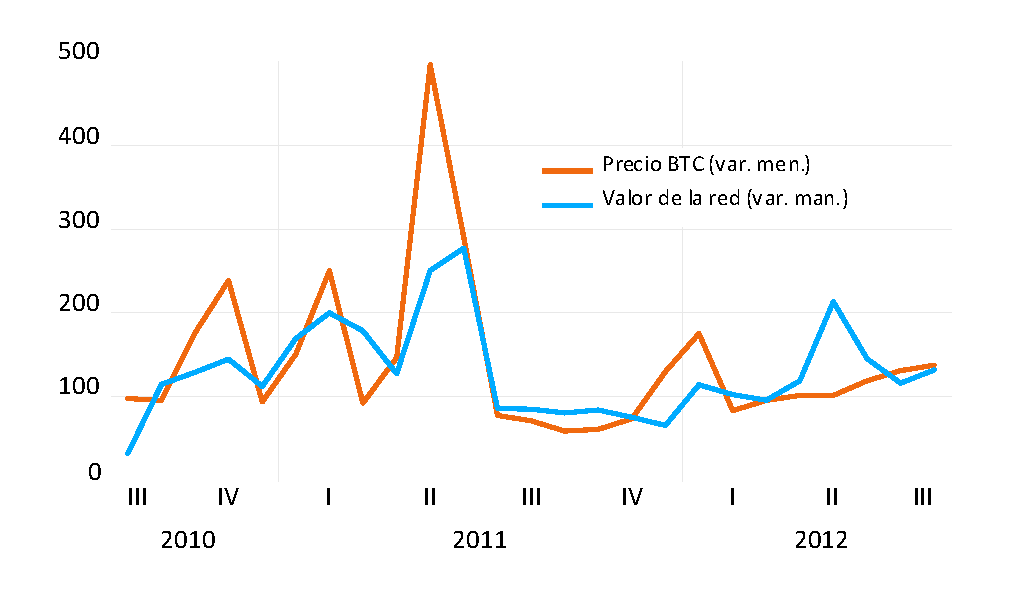
\includegraphics[width=1\textwidth]{images/C2/c2_var_men_timesseries_presentacion.pdf}
     \end{center}
\end{figure}

\note{
\begin{itemize}
    \item Luego de generar la serie temporal, se toma la serie en variaciones para dar cuenta del crecimiento poblacional "n". 
\end{itemize}
}

\end{frame}
%----------

% comparación con referencias actuales

\begin{frame}
\frametitle{Estos resultados se encuentran asociados a nuevas métricas de mercado}

\begin{figure}[H]
    \begin{center}
         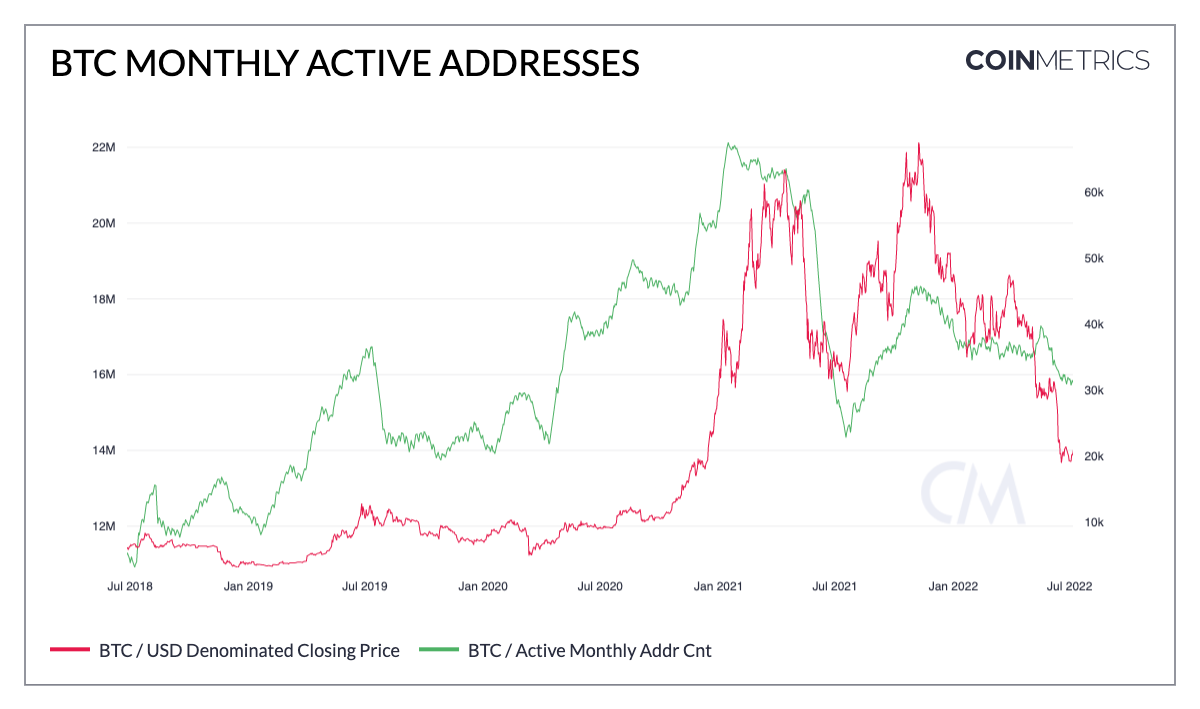
\includegraphics[width=1\textwidth]{images/C2/ref/coinmetrics_addr.png}
     \end{center}
\end{figure}

\note{
\begin{itemize}
    \item Este tipo de análisis a partir de datos de la cadena de bloques están comenzando a ser utilizados por consultoras de mercado para evaluar la evolución del precio de bitcoin y otros activos digitales. 
    \item Este es un indicador de la empresa Glassnode, donde se asocian las nuevas direcciones utilizadas en la red bitcoin al valor de mercado del bitcoin. 
\end{itemize}
}

\end{frame}
%----------

\begin{frame}
\frametitle{Estos resultados se encuentran asociados a nuevas métricas de mercado}

\begin{figure}[H]
    \begin{center}
         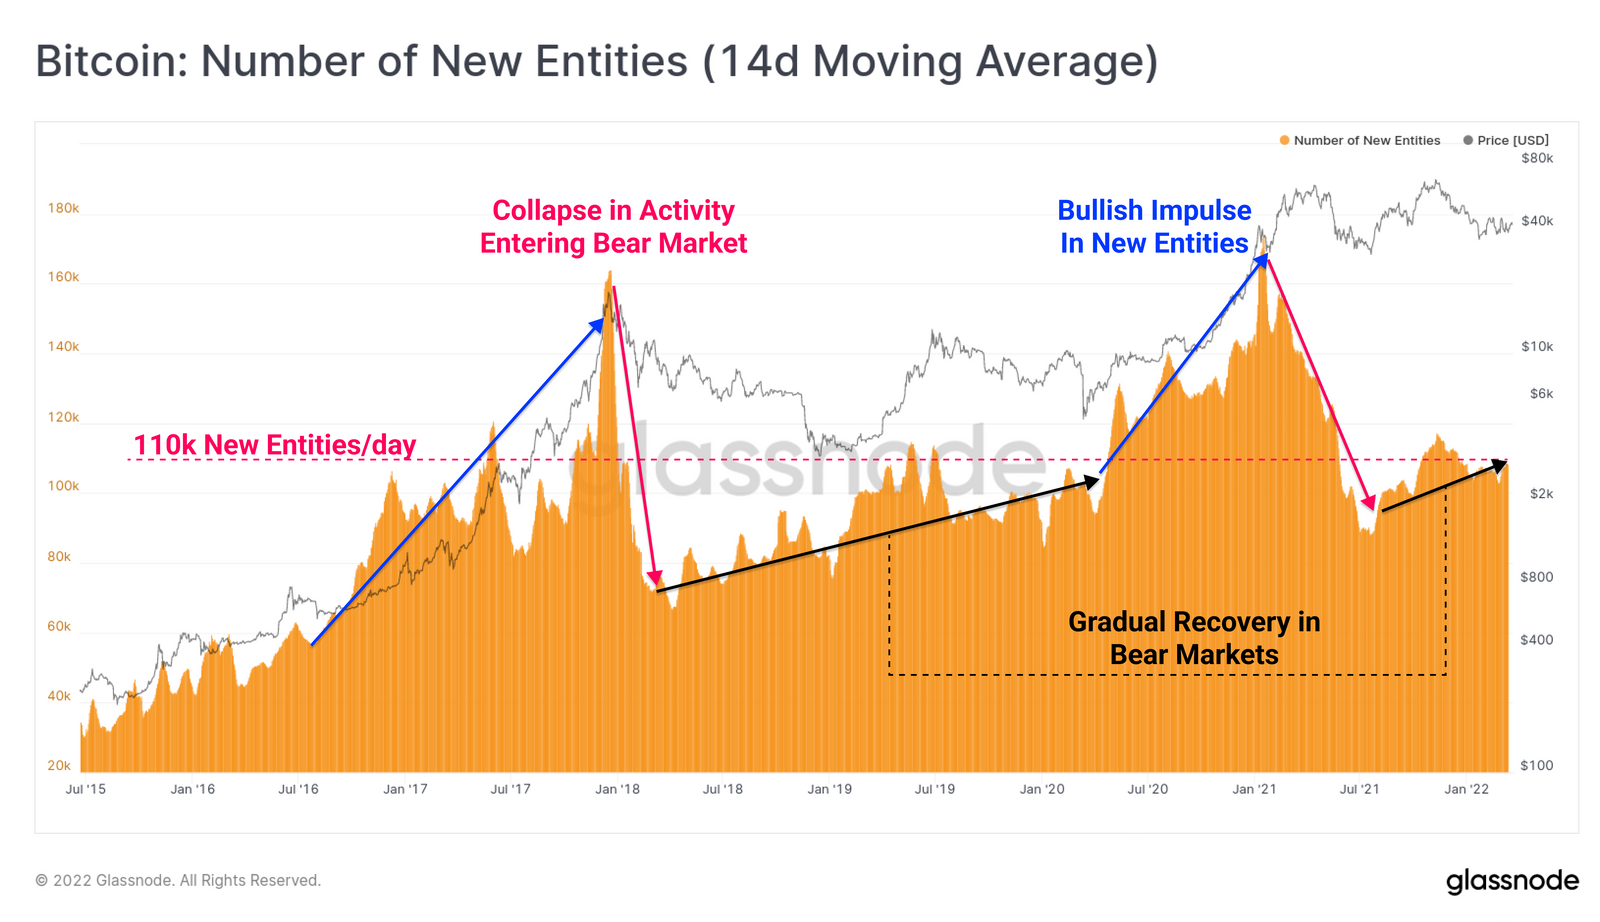
\includegraphics[width=1\textwidth]{images/C2/ref/07_newentities.png}
     \end{center}
\end{figure}

\note{
\begin{itemize}
    \item Este tipo de análisis a partir de datos de la cadena de bloques están comenzando a ser utilizados por consultoras de mercado para evaluar la evolución del precio de bitcoin y otros activos digitales. 
    \item Este es un indicador de la empresa Glassnode, donde se asocian las nuevas direcciones utilizadas en la red bitcoin al valor de mercado del bitcoin. 
\end{itemize}
}

\end{frame}
%----------

\begin{frame}{}

    \vspace{5mm}
    \begin{itemize}
        \setlength\itemsep{1em}
        \item[] La \textcolor{blue}{\textbf{conclusión principal}} es que \textcolor{blue}{bitcoin es una tecnología funcionalmente equivalente al dinero}.  
        \item[] La \textcolor{dgreen}{\textbf{evaluación conceptual}} corrobora la conjetura a partir de la introducción de la DLT en el modelo de generaciones superpuestas de manera directa como un \textcolor{dgreen}{sistema de registros público} y como \textcolor{dgreen}{memoria}.
        \item[] La \textcolor{orange}{\textbf{evaluación empírica}} corrobora la conjetura a partir de la \textcolor{orange}{construcción de una cadena de operaciones que simula al modelo} teórico.
    \end{itemize}

\note{
\begin{itemize}
    \item Luego de realizar la evaluación conceptual y empírica en esta primera parte de la investigación, se  llega a las siguientes conclusiones: (leer filmina)
\end{itemize}
}
    
\end{frame}
%----------
